% !TEX program = xelatex
% Шаблон научной статьи НИТУ «МИСиС»

\documentclass{misisarticle}

\usepackage{tikz}
\usetikzlibrary{arrows.meta, positioning, calc}

\grnti{28.23.27, 55.30.31, 28.23.25}
\asjc{1702, 2207}
\oecd{1.02, 2.02}

\title{Разработка модели прогнозирования отказов RL-политики толкания по форме объекта и её применение для формирования учебного плана}

\misisauthor{Б.~А.~Кузнечик}{кафедра инженерной кибернетики НИТУ «МИСиС»}{Москва, Россия}{m2308277@edu.misis.ru}

\abstract{%
  Рассматривается задача перемещения толканием объекта произвольной, в том числе невыпуклой, формы в заданную позицию и ориентацию на плоскости. Управление обучается методом обучения с подкреплением в симуляции. Обученная политика на одних формах работает надёжно, а на других систематически ошибается, и известные методы обнаруживают это только во время выполнения. Предлагается лёгкая модель, которая до начала толкания по контуру объекта оценивает вероятность неудачи политики с учётом достигнутого ею уровня обучения. Входами служат геометрические признаки формы: доля невыпуклости, вытянутость, число вогнутостей контура, отношение моментов инерции и индекс сложности набора EGAD. Сравниваются логистическая регрессия, градиентный бустинг и небольшая нейросеть по точкам контура. Обучающие данные собираются автоматически: контрольные точки политики PPO многократно запускаются в MuJoCo на формах, которых политика не видела. Прогноз используется для учебного плана: при обучении новой политики чаще предъявляются формы с прогнозом неудачи около 50\%. Описана методика проверки на отложенных формах по ROC-AUC, оценке Брайера и ошибке калибровки, а также сравнения учебного плана со случайным выбором форм и с Prioritized Level Replay.
}

\keywords{%
  обучение с подкреплением, толкание объектов по плоскости, прогнозирование отказов, геометрические дескрипторы формы, учебный план, объекты произвольной формы
}

\begin{document}

\maketitle

% ============================================================
\section{Введение}

Толкание позволяет роботу перемещать предметы, которые слишком велики, тяжелы или неудобны для захвата, а также точно подправлять положение объекта перед следующей операцией. Результат толчка зависит от формы объекта, трения и распределения массы, причём эти параметры известны неточно~\cite{mason1986, lynch1996}. Поэтому управление толканием всё чаще обучают с подкреплением в симуляции~\cite{li2018, cong2022}.

Средняя доля успешных попыток скрывает важную особенность таких политик: на разных формах качество различается. С вытянутым или вогнутым объектом политика может раз за разом проворачивать его мимо цели, тогда как компактные выпуклые объекты она перемещает без затруднений. Отсюда возникают две практические проблемы. Во-первых, перед запуском неизвестно, можно ли доверить политике данный объект или лучше выбрать другую стратегию. Во-вторых, объекты для обучения обычно выбираются случайно, и часть времени тратится на формы, которые для агента на текущем этапе либо тривиальны, либо пока непосильны.

Обе проблемы сводятся к одному вопросу: можно ли по геометрии объекта заранее оценить вероятность неудачи политики? Настоящая работа посвящена разработке такой оценки. Вклад работы состоит в следующем:
\begin{itemize}
  \item предложена модель априорного прогноза вероятности неудачи RL-политики толкания, использующая только геометрию объекта и уровень обучения политики;
  \item на основе прогноза построен способ формирования учебного плана, не требующий запусков среды для оценки сложности каждой формы;
  \item описана процедура получения открытого набора данных «форма объекта~--- доля неудач политики», собираемого в симуляции.
\end{itemize}

В статье изложены анализ работ, постановка задачи и описание методов. Эксперименты на момент написания ещё не проведены, поэтому в разделе~\ref{sec:methods} приведена методика их проведения, а численные результаты не приводятся.

% ============================================================
\section{Анализ работ}

\subsection{Толкание объектов произвольной формы}

Классические работы описывают толкание аналитически: определяют направление вращения объекта и условия устойчивого толкания при известных форме и трении~\cite{mason1986, lynch1996}. Такие модели наглядны, но опираются на параметры, которые на практике приходится оценивать.

Обучаемые методы снимают это требование. Push-Net~\cite{li2018} предсказывает толчки по изображениям с помощью рекуррентной сети, которая учитывает историю взаимодействия с объектом и оценивает положение его центра масс. Рекуррентные модели, обучаемые в симуляции, рассматриваются и в~\cite{cong2020}. В~\cite{cong2022} состояние строится из сжатого вариационным автокодировщиком изображения и положения схвата, а политика обучается методом Soft Actor-Critic. В~\cite{wang2023} информация о контакте включена в функцию награды, что повышает долю успехов на незнакомых объектах. Толкание среди препятствий изучается в~\cite{dengler2022, luz2025}. В недавней работе~\cite{yuan2026} политика предсказывает контактные действия по нормализованному облаку точек, а каждое предложенное действие проверяется по оценке устойчивости.

Эти работы повышают качество политики, но вопрос о том, какие именно формы окажутся трудными и можно ли определить это заранее, в них не является предметом исследования. Набор EGAD~\cite{morrison2020} даёт сетку форм по двум осям: морфологической сложности (энтропия распределения угловых дефектов вершин) и трудности захвата (75-й перцентиль качества сэмплированных захватов). Вторая ось определена именно для захвата, поэтому она не обязана отражать трудность толкания. Связь геометрических мер с неудачами при толкании составляет один из предметов данной работы.

\subsection{Учебные планы в обучении с подкреплением}

Учебный план задаёт порядок предъявления задач агенту~\cite{portelas2020}. Автоматические планы подбирают задачи под текущие возможности агента. В~\cite{florensa2018} генератор предлагает цели промежуточной трудности: не слишком лёгкие и не слишком сложные для текущей политики. Prioritized Level Replay (PLR)~\cite{jiang2021} выбирает для повторения уровни, на которых ожидается наибольший прирост обучения, оценивая их по ошибке функции ценности. Для такой оценки уровень нужно хотя бы раз сыграть, а его геометрия не используется.

Геометрию объекта учитывают работы по манипулированию. В UniDexGrasp++~\cite{wan2023} задачи захвата многопалой рукой упорядочиваются с учётом геометрических признаков объектов. В~\cite{zhang2023} навык манипулирования в руке переносится на сложную форму через цепочку промежуточных форм. В~\cite{huang2026} для совместного толкания и захвата этапы плана различаются плотностью загромождения и трудностью объектов. Общим для них является то, что сложность определяется заранее заданным правилом или группировкой, а не обучаемым прогнозом неудачи конкретной политики.

Отметим также связанные работы из сборника кафедры. В~\cite{kiselev2025} на примере выбора траектории и перестроения в симуляции сравниваются Rainbow DQN и графовая сеть на основе Double DQN; сравнение алгоритмов в управляемой среде близко к используемому здесь подходу. В~\cite{savelyev2025} описан модуль голосового управления манипулятором на основе большой языковой модели: при таком управлении команду формулирует человек, и оценка выполнимости команды до её исполнения была бы полезна.

\subsection{Прогнозирование отказов}

Предсказание отказов обученных политик активно развивается, но в основном как мониторинг во время выполнения. Sentinel~\cite{agia2024} обнаруживает отказы по временной согласованности действий и по анализу видео языковой моделью. FAIL-Detect~\cite{xu2025} и FIPER~\cite{romer2025} не требуют примеров отказов; FIPER сочетает обнаружение нетипичных наблюдений с оценкой неопределённости действий и калибрует пороги на успешных запусках. Эти методы рассчитаны на политики имитационного обучения и получают сигнал уже в ходе исполнения.

В табл.~\ref{tab:related} работы сопоставлены с предлагаемым подходом. В просмотренной литературе не найдено работ, где вероятность неудачи RL-политики толкания прогнозировалась бы до выполнения только по геометрии объекта. Этот вывод основан на ограниченном поиске и будет уточняться.

\begin{table}[htbp]
  \caption{Сопоставление с близкими работами}
  \label{tab:related}
  \centering
  \small
  \begin{tabular}{>{\raggedright\arraybackslash}p{0.32\columnwidth}>{\raggedright\arraybackslash}p{0.25\columnwidth}>{\raggedright\arraybackslash}p{0.28\columnwidth}}
    \toprule
    \textbf{Работа} & \textbf{Что оценивается} & \textbf{Когда и по чему} \\
    \midrule
    Sentinel, FAIL-Detect, FIPER~\cite{agia2024, xu2025, romer2025} & Отказ политики & При выполнении, по наблюдениям и действиям \\
    EGAD~\cite{morrison2020} & Трудность захвата & Заранее, по геометрии \\
    PLR~\cite{jiang2021} & Польза уровня & После запуска, по ошибке ценности \\
    UniDexGrasp++~\cite{wan2023} & Порядок задач & Заранее, по геометрии \\
    Предлагаемый подход & Вероятность отказа толкания & Заранее, по геометрии и уровню политики \\
    \bottomrule
  \end{tabular}
\end{table}

% ============================================================
\section{Постановка задачи}

На столе лежит объект формы $s$ из множества форм $\mathcal{S}$. Его физические параметры $\xi$ (коэффициент трения, масса, положение центра масс) точно не известны. Состояние сцены включает позу объекта $q_t = (x_t, y_t, \theta_t)$ и положение толкателя $p_t \in \mathbb{R}^2$ (рис.~\ref{fig:scene}). Цель эпизода~--- поза $q^{*}$. На каждом шаге политика $\pi$ задаёт смещение толкателя $a_t \in [-\delta, \delta]^2$.

Эпизод считается успешным, если не позднее шага $T$ одновременно выполнены условия
\begin{equation}
  \|(x_t, y_t) - (x^{*}, y^{*})\| \le \varepsilon_p, \quad
  |\mathrm{wrap}(\theta_t - \theta^{*})| \le \varepsilon_\theta,
  \label{eq:success}
\end{equation}
где $\mathrm{wrap}$ приводит угол к диапазону $(-\pi, \pi]$. Если условия не выполнены или объект покинул рабочую зону, фиксируется неудача: $Y = 1$.

\begin{figure}[htbp]
  \centering
  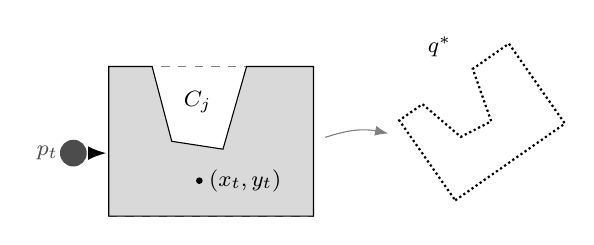
\begin{tikzpicture}[x=1cm, y=1cm, font=\footnotesize]
    \draw[dashed, gray] (0,0) -- (2.6,0) -- (2.6,1.9) -- (0,1.9) -- cycle;
    \fill[gray!30, draw=black]
      (0,0) -- (2.6,0) -- (2.6,1.9) -- (1.75,1.9) -- (1.45,0.85) -- (0.8,0.95) -- (0.55,1.9) -- (0,1.9) -- cycle;
    \fill (1.15,0.45) circle (1.2pt) node[right] {$(x_t,y_t)$};
    \node at (1.13,1.45) {$C_j$};
    \fill[black!70] (-0.45,0.8) circle (0.17) node[left=2pt] {$p_t$};
    \draw[-{Latex}, thick] (-0.27,0.8) -- (-0.03,0.8);
    \begin{scope}[shift={(4.4,0.2)}, rotate=35]
      \draw[thick, densely dotted]
        (0,0) -- (1.7,0) -- (1.7,1.24) -- (1.14,1.24) -- (0.95,0.56) -- (0.52,0.62) -- (0.36,1.24) -- (0,1.24) -- cycle;
    \end{scope}
    \node at (4.2,2.15) {$q^{*}$};
    \draw[-{Latex}, gray] (2.75,1.0) to[bend left=15] (3.55,1.05);
  \end{tikzpicture}
  \caption{Сцена толкания: контур объекта, выпуклая оболочка (штриховая линия), вогнутость $C_j$, толкатель и целевая поза (пунктир)}
  \label{fig:scene}
\end{figure}

Для политики $\pi$ определим вероятность неудачи на форме $s$:
\begin{equation}
  F_\pi(s) = \mathbb{P}\left[\,Y = 1 \mid s, \pi\,\right],
  \label{eq:failure}
\end{equation}
где вероятность берётся по распределениям параметров $\xi$, начальных поз и целей. Требуется построить вычислительно лёгкую функцию $g_\phi$, которая до начала эпизода оценивает~\eqref{eq:failure} по описанию формы $\mathbf{x}(s)$ и уровню обучения политики $c \in [0, 1]$:
\begin{equation}
  g_\phi(\mathbf{x}(s), c) \approx F_{\pi_c}(s).
  \label{eq:target}
\end{equation}
Запуск среды при вычислении прогноза не допускается. Оценка должна быть качественной на формах, не участвовавших ни в обучении политики, ни в обучении $g_\phi$, и откалиброванной: значение $0{,}7$ должно соответствовать примерно 70\% неудач.

Вторая задача~--- использовать $g_\phi$ для выбора форм при обучении новой политики так, чтобы сократить число шагов до заданной доли успехов на новых формах по сравнению со случайным выбором.

% ============================================================
\section{Описание методов}
\label{sec:methods}

Общая схема показана на рис.~\ref{fig:pipeline}. Значения параметров, приведённые ниже, являются исходными и будут уточняться в пробных запусках.

\begin{figure}[htbp]
  \centering
  \begin{tikzpicture}[
      font=\footnotesize,
      box/.style={draw, rounded corners=1.5pt, align=center, minimum width=0.86\columnwidth, inner sep=3pt},
      arr/.style={-{Latex}, thick}]
    \node[box] (a) {Обучение базовой политики PPO на $\mathcal{S}_\pi$,\\контрольные точки $\pi_{c}$ разных уровней};
    \node[box, below=4mm of a] (b) {Запуски $\pi_{c}$ на $\mathcal{S}_g$: доли неудач $\hat{F}(s, c)$};
    \node[box, below=4mm of b] (c) {Признаки формы $\mathbf{x}(s)$ и обучение модели прогноза $g_\phi$};
    \node[box, below=4mm of c] (d) {Проверка прогноза на $\mathcal{S}_t$: ROC-AUC, оценка Брайера, ECE};
    \node[box, below=4mm of d] (e) {Учебный план: новая политика, выбор форм из $\mathcal{S}_\pi$ по $g_\phi$};
    \node[box, below=4mm of e] (f) {Сравнение планов на $\mathcal{S}_t$ и формах YCB};
    \draw[arr] (a) -- (b);
    \draw[arr] (b) -- (c);
    \draw[arr] (c) -- (d);
    \draw[arr] (d) -- (e);
    \draw[arr] (e) -- (f);
  \end{tikzpicture}
  \caption{Этапы предлагаемого метода}
  \label{fig:pipeline}
\end{figure}

\subsection{Среда и объекты}

Среда реализуется в симуляторе MuJoCo~\cite{mujoco2012}, который рассчитан на контактную динамику и работает без видеокарты. Вместо полного манипулятора используется цилиндрический толкатель радиусом 1~см, перемещаемый по плоскости с малой скоростью. Такое упрощение отделяет исследуемую зависимость от формы от кинематики конкретной руки.

Формы берутся из набора EGAD~\cite{morrison2020}: 2282 обучающие модели на сетке $25 \times 25$ и 49 оценочных. Поскольку задача плоская, модель заменяется призмой. Контур $P$~--- внешняя граница проекции модели на стол в устойчивом положении, затем контур масштабируется к общему наибольшему размеру 12~см. Благодаря этому геометрия контакта однозначно задаётся контуром.

Важная техническая особенность: при расчёте столкновений MuJoCo заменяет каждую сетку её выпуклой оболочкой, и вогнутости объекта исчезают. Поэтому невыпуклые призмы заранее разбиваются на выпуклые части алгоритмом CoACD~\cite{coacd2022}, и каждая часть подключается отдельной геометрией. Для проверки переносимости на формы другого происхождения используется часть объектов набора YCB.

\subsection{Базовая политика}

Наблюдение содержит цель и положение толкателя в системе координат объекта, а также 32 равномерно расположенные точки контура. Обозначим через $d_t$ сумму нормированных ошибок по позиции и углу. Награда имеет вид
\begin{equation}
  r_t = \alpha (d_{t-1} - d_t) - \beta\,\mathrm{dist}(p_t, P_t) + R\,\mathbf{1}[\text{успех}],
  \label{eq:reward}
\end{equation}
где второе слагаемое приближает толкатель к объекту, а $P_t$~--- контур объекта на шаге $t$.

Политика обучается алгоритмом PPO~\cite{ppo2017} в реализации Stable-Baselines3~\cite{sb3} на многоядерном процессоре с параллельными средами. Трение, масса и центр масс рандомизируются в каждом эпизоде~\cite{peng2018}. В ходе обучения сохраняются контрольные точки $\pi_c$. Уровень $c$ определяется как доля успехов политики на фиксированном проверочном наборе форм. Обучение повторяется с пятью начальными значениями генератора, чтобы прогноз описывал трудность формы, а не особенности одного запуска.

\subsection{Сбор данных и разбиение форм}

Формы делятся на три непересекающихся множества, стратифицированных по ячейкам сетки EGAD: $\mathcal{S}_\pi$ для обучения политики, $\mathcal{S}_g$ для обучения прогноза и $\mathcal{S}_t$ для итоговой проверки. Это принципиально: на формах из обучения политика работает лучше, поэтому метки на них описывали бы другую величину, а разделение только по эпизодам привело бы к утечке данных между выборками.

Каждая контрольная точка запускается на каждой форме из $\mathcal{S}_g$ в $N$ эпизодах со случайными параметрами, начальными позами и целями. Оценкой~\eqref{eq:failure} служит доля неудач $\hat{F}(s, c) = k_{s,c}/N$, где $k_{s,c}$~--- число неудач. Полученная таблица публикуется вместе с кодом.

\subsection{Геометрические признаки}

По контуру $P$ вычисляются признаки из табл.~\ref{tab:features}. Здесь $A(\cdot)$~--- площадь, $\mathrm{CH}(P)$~--- выпуклая оболочка, $\lambda_{\min} \le \lambda_{\max}$~--- собственные значения ковариационной матрицы точек области, $I_z$~--- полярный момент инерции области при единичной плотности. Величина $A^2/(2\pi)$ равна полярному моменту круга той же площади, поэтому для круга отношение моментов равно единице. Вогнутостями считаются связные компоненты $C_j$ области $\mathrm{CH}(P) \setminus P$ площадью не менее 1\% от $A(P)$.

\begin{table}[htbp]
  \caption{Геометрические признаки формы}
  \label{tab:features}
  \centering
  \begin{tabular}{>{\raggedright\arraybackslash}p{0.46\columnwidth}l}
    \toprule
    \textbf{Признак} & \textbf{Формула} \\
    \midrule
    Доля невыпуклости & $1 - A(P)/A(\mathrm{CH}(P))$ \\
    Вытянутость & $1 - \sqrt{\lambda_{\min}/\lambda_{\max}}$ \\
    Число вогнутостей контура & $|\{C_j\}|$ \\
    Отношение моментов инерции & $2\pi I_z / A(P)^2$ \\
    Индекс сложности EGAD & номер по оси сложности \\
    \bottomrule
  \end{tabular}
\end{table}

\subsection{Модель прогноза}

Рассматриваются три модели возрастающей сложности: логистическая регрессия по признакам $\mathbf{x}(s)$, уровню $c$ и их произведениям; градиентный бустинг LightGBM~\cite{lightgbm2017} по тем же входам; небольшая нейросеть по 128 точкам контура, приведённым к главным осям. Последняя устроена по образцу PointNet~\cite{pointnet2017}: общая для всех точек сеть и симметричная агрегация делают результат независимым от выбора начальной точки. К вектору формы добавляется уровень $c$.

Модели обучаются минимизацией отрицательного логарифма биномиального правдоподобия:
\begin{equation}
  \mathcal{L}(\phi) = -\sum_{s, c} \left[ k_{s,c} \ln g_\phi + (N - k_{s,c}) \ln (1 - g_\phi) \right],
  \label{eq:loss}
\end{equation}
где $g_\phi = g_\phi(\mathbf{x}(s), c)$. Гиперпараметры подбираются кросс-валидацией с группировкой по формам.

\subsection{Учебный план на основе прогноза}

Целевая доля неудач $p^{*} = 0{,}5$ соответствует идее задач промежуточной трудности~\cite{florensa2018}: лёгкие формы дают мало нового, а безнадёжные почти не дают полезного сигнала. При обучении новой политики её уровень $c$ периодически измеряется на проверочном наборе, и для каждой формы из $\mathcal{S}_\pi$ вычисляется вес
\begin{equation}
  w_c(s) = \exp\left( -\frac{\left(g_\phi(\mathbf{x}(s), c) - p^{*}\right)^2}{2\sigma^2} \right).
  \label{eq:weight}
\end{equation}
Форма для следующего эпизода выбирается с вероятностью
\begin{equation}
  P_c(s) = (1 - \eta) \frac{w_c(s)}{\sum_{s'} w_c(s')} + \frac{\eta}{|\mathcal{S}_\pi|},
  \label{eq:sampling}
\end{equation}
где равномерная добавка $\eta$ не даёт политике забывать остальные формы (исходные значения $\sigma = 0{,}15$, $\eta = 0{,}2$). Зависимость прогноза от $c$ здесь необходима: при статическом прогнозе одни и те же формы оставались бы в выборе на всём протяжении обучения. По мере роста $c$ прогноз снижается, и к порогу $p^{*}$ подходят всё более сложные формы.

В отличие от PLR~\cite{jiang2021}, план не требует предварительного запуска формы и применим к новым формам сразу. Его ограничение в том, что $g_\phi$ обучена на политиках со случайным выбором форм, тогда как политика с учебным планом накапливает другой опыт. Поэтому калибровка прогноза проверяется и в ходе обучения по учебному плану.

\subsection{Методика оценки}

\textit{Качество прогноза} оценивается на $\mathcal{S}_t$ при $N = 50$. Форма считается трудной при $\hat{F} \ge 0{,}5$; способность отличать такие формы измеряется ROC-AUC. Точность вероятностей оценивается мерой Брайера~\cite{brier1950} и ожидаемой ошибкой калибровки ECE~\cite{guo2017}:
\begin{align}
  \mathrm{BS} &= \frac{1}{|\mathcal{S}_t|} \sum_{s} \left( g_\phi(\mathbf{x}(s), c) - \hat{F}(s, c) \right)^2, \label{eq:brier} \\
  \mathrm{ECE} &= \sum_{b=1}^{10} \frac{|B_b|}{|\mathcal{S}_t|} \left| \overline{g}_{B_b} - \overline{\hat{F}}_{B_b} \right|, \label{eq:ece}
\end{align}
где $B_b$~--- формы, попавшие в $b$-й интервал по значению прогноза. Базовыми методами служат порог по одной мере сложности и индекс EGAD. Вклад признаков определяется перестановочной важностью, а связь каждой меры с неудачами~--- коэффициентом ранговой корреляции Спирмена.

\textit{Учебный план} сравнивается со случайным выбором форм, с PLR~\cite{jiang2021} и с вариантом статического прогноза без учёта $c$. Метрики: доля успешных перемещений на $\mathcal{S}_t$ и формах YCB, итоговые ошибки по позиции и углу, число шагов обучения до заданной доли успехов. Для каждого варианта выполняется пять запусков; доверительные интервалы строятся бутстрэпом.

Проверяются две гипотезы: прогноз по совокупности признаков превосходит любую одиночную меру сложности, а учебный план сокращает число шагов до заданной доли успехов без снижения итогового качества. Если вторая гипотеза не подтвердится, прогноз сохранит самостоятельную ценность для оценки применимости политики к новому объекту. Перенос на реальный объект в данной работе не рассматривается; на реальном стенде контур мог бы получаться по данным сенсоров, и повышение плотности облака точек механического лидара с помощью виртуального зеркального канала рассмотрено в~\cite{vishnevsky2026}.

% ============================================================
\begin{thebibliography}{99}

\bibitem{mason1986} M. T. Mason, “Mechanics and planning of manipulator pushing operations,” \textit{The International Journal of Robotics Research}, vol.~5, no.~3, pp.~53--71, 1986, doi: 10.1177/027836498600500303.

\bibitem{lynch1996} K. M. Lynch and M. T. Mason, “Stable pushing: Mechanics, controllability, and planning,” \textit{The International Journal of Robotics Research}, vol.~15, no.~6, pp.~533--556, 1996, doi: 10.1177/027836499601500602.

\bibitem{li2018} J. K. Li, W. S. Lee, and D. Hsu, “Push-Net: Deep planar pushing for objects with unknown physical properties,” in \textit{Robotics: Science and Systems XIV}, 2018, doi: 10.15607/RSS.2018.XIV.024.

\bibitem{cong2022} L. Cong, H. Liang, P. Ruppel, Y. Shi, M. Görner, N. Hendrich, and J. Zhang, “Reinforcement learning with vision-proprioception model for robot planar pushing,” \textit{Frontiers in Neurorobotics}, vol.~16, 2022, doi: 10.3389/fnbot.2022.829437.

\bibitem{cong2020} L. Cong, M. Görner, P. Ruppel, H. Liang, N. Hendrich, and J. Zhang, “Self-adapting recurrent models for object pushing from learning in simulation,” in \textit{2020 IEEE/RSJ International Conference on Intelligent Robots and Systems (IROS)}, 2020, pp.~5304--5310, doi: 10.1109/IROS45743.2020.9341076.

\bibitem{wang2023} S. Wang, L. Sun, F. Zha, W. Guo, and P. Wang, “Learning adaptive reaching and pushing skills using contact information,” \textit{Frontiers in Neurorobotics}, vol.~17, 2023, doi: 10.3389/fnbot.2023.1271607.

\bibitem{dengler2022} N. Dengler, D. Großklaus, and M. Bennewitz, “Learning goal-oriented non-prehensile pushing in cluttered scenes,” in \textit{2022 IEEE/RSJ International Conference on Intelligent Robots and Systems (IROS)}, 2022, pp.~1116--1122, doi: 10.1109/IROS47612.2022.9981873.

\bibitem{luz2025} G. S. Luz and D. G. Macharet, “A DRL approach for mapless planar pushing of arbitrary objects in cluttered environments,” SBC OpenLib, 2025. [Online]. Available: \url{https://sol.sbc.org.br/index.php/sbrlars_estendido/article/download/39152/38924/}

\bibitem{yuan2026} Z. Yuan, T. Hu, A. Xiao, Y. Deng, D. Hsu, and H. Zhang, “Receding-horizon pushing with composable object-centric policies,” arXiv:2609.23439, 2026.

\bibitem{morrison2020} D. Morrison, P. Corke, and J. Leitner, “EGAD! An evolved grasping analysis dataset for diversity and reproducibility in robotic manipulation,” \textit{IEEE Robotics and Automation Letters}, vol.~5, no.~3, pp.~4368--4375, 2020, doi: 10.1109/LRA.2020.2992195.

\bibitem{portelas2020} R. Portelas, C. Colas, L. Weng, K. Hofmann, and P.-Y. Oudeyer, “Automatic curriculum learning for deep RL: A short survey,” in \textit{Proc. 29th International Joint Conference on Artificial Intelligence (IJCAI)}, 2020, pp.~4819--4825, doi: 10.24963/ijcai.2020/671.

\bibitem{florensa2018} C. Florensa, D. Held, X. Geng, and P. Abbeel, “Automatic goal generation for reinforcement learning agents,” in \textit{Proc. 35th International Conference on Machine Learning}, PMLR, vol.~80, 2018, pp.~1515--1528.

\bibitem{jiang2021} M. Jiang, E. Grefenstette, and T. Rocktäschel, “Prioritized level replay,” in \textit{Proc. 38th International Conference on Machine Learning}, PMLR, vol.~139, 2021, pp.~4940--4950.

\bibitem{wan2023} W. Wan et al., “UniDexGrasp++: Improving dexterous grasping policy learning via geometry-aware curriculum and iterative generalist-specialist learning,” in \textit{2023 IEEE/CVF International Conference on Computer Vision (ICCV)}, 2023, pp.~3868--3879, doi: 10.1109/ICCV51070.2023.00360.

\bibitem{zhang2023} Y. Zhang, A. Clegg, S. Ha, G. Turk, and Y. Ye, “Learning to transfer in-hand manipulations using a greedy shape curriculum,” \textit{Computer Graphics Forum}, vol.~42, no.~2, pp.~25--36, 2023, doi: 10.1111/cgf.14741.

\bibitem{huang2026} C. Huang, A. Efendi, and Y. Wang, “Curriculum-guided deep reinforcement learning with fuzzy rewards for autonomous push-grasp manipulation in cluttered environments,” \textit{Robotics and Autonomous Systems}, vol.~198, art.~105325, 2026, doi: 10.1016/j.robot.2025.105325.

\bibitem{kiselev2025} С. Д. Киселев, А. В. Алтунян, «Локальные методы планирования траекторий на основе обучения с подкреплением», в сб. \textit{Искусственный интеллект в промышленных, коммерческих, медицинских и финансовых приложениях}, вып.~3. М.: НИТУ «МИСИС», 2025, с.~84--89.

\bibitem{savelyev2025} Я. С. Савельев, И. А. Рябухин, Т. А. Синельникова, «Применение больших языковых моделей в рамках голосового управления роботом-манипулятором посредством естественной речи», в сб. \textit{Искусственный интеллект в промышленных, коммерческих, медицинских и финансовых приложениях}, вып.~3. М.: НИТУ «МИСИС», 2025, с.~116--119.

\bibitem{agia2024} C. Agia, R. Sinha, J. Yang, Z. Cao, R. Antonova, M. Pavone, and J. Bohg, “Unpacking failure modes of generative policies: Runtime monitoring of consistency and progress,” in \textit{Conference on Robot Learning (CoRL)}, 2024, arXiv:2410.04640.

\bibitem{xu2025} C. Xu et al., “Can we detect failures without failure data? Uncertainty-aware runtime failure detection for imitation learning policies,” arXiv:2503.08558, 2025.

\bibitem{romer2025} R. Römer, A. Kobras, L. Worbis, and A. P. Schoellig, “Failure prediction at runtime for generative robot policies,” in \textit{Advances in Neural Information Processing Systems (NeurIPS)}, 2025, arXiv:2510.09459.

\bibitem{mujoco2012} E. Todorov, T. Erez, and Y. Tassa, “MuJoCo: A physics engine for model-based control,” in \textit{2012 IEEE/RSJ International Conference on Intelligent Robots and Systems}, 2012, pp.~5026--5033, doi: 10.1109/IROS.2012.6386109.

\bibitem{coacd2022} X. Wei, M. Liu, Z. Ling, and H. Su, “Approximate convex decomposition for 3D meshes with collision-aware concavity and tree search,” \textit{ACM Transactions on Graphics}, vol.~41, no.~4, pp.~1--18, 2022, doi: 10.1145/3528223.3530103.

\bibitem{ppo2017} J. Schulman, F. Wolski, P. Dhariwal, A. Radford, and O. Klimov, “Proximal policy optimization algorithms,” arXiv:1707.06347, 2017.

\bibitem{sb3} A. Raffin, A. Hill, A. Gleave, A. Kanervisto, M. Ernestus, and N. Dormann, “Stable-Baselines3: Reliable reinforcement learning implementations,” \textit{Journal of Machine Learning Research}, vol.~22, no.~268, pp.~1--8, 2021.

\bibitem{peng2018} X. B. Peng, M. Andrychowicz, W. Zaremba, and P. Abbeel, “Sim-to-real transfer of robotic control with dynamics randomization,” in \textit{2018 IEEE International Conference on Robotics and Automation (ICRA)}, 2018, pp.~3803--3810, doi: 10.1109/ICRA.2018.8460528.

\bibitem{lightgbm2017} G. Ke et al., “LightGBM: A highly efficient gradient boosting decision tree,” in \textit{Advances in Neural Information Processing Systems}, vol.~30, 2017.

\bibitem{pointnet2017} C. R. Qi, H. Su, K. Mo, and L. J. Guibas, “PointNet: Deep learning on point sets for 3D classification and segmentation,” in \textit{2017 IEEE Conference on Computer Vision and Pattern Recognition (CVPR)}, 2017, pp.~77--85, doi: 10.1109/CVPR.2017.16.

\bibitem{brier1950} G. W. Brier, “Verification of forecasts expressed in terms of probability,” \textit{Monthly Weather Review}, vol.~78, no.~1, pp.~1--3, 1950.

\bibitem{guo2017} C. Guo, G. Pleiss, Y. Sun, and K. Q. Weinberger, “On calibration of modern neural networks,” in \textit{Proc. 34th International Conference on Machine Learning}, PMLR, vol.~70, 2017, pp.~1321--1330.

\bibitem{vishnevsky2026} М. Р. Вишневский, И. Ю. Фёдоров, «Повышение пространственного разрешения механических LiDAR-систем с использованием виртуального зеркального канала и автоматической калибровки», \textit{Труды Института системного программирования РАН}, т.~38, вып.~3, с.~101--114, 2026, doi: 10.15514/ISPRAS-2026-38(3)-38.

\end{thebibliography}

\end{document}
